\section{Motivation}
\label{sec:motivation}
Real-time control of autonomous vehicles requires the processing of a large amount of sensor data, which is used by the vehicle to determine its position in the world and to calculate its next move.
Examples include data from cameras, LIDAR, radars and ultrasound radars, and possibly information communicated by other vehicles or the road infrastructure.
Google's autonomous vehicles generate over 750MB/s of sensor data ~\cite{diamandis2015bold} which must be processed by the perception pipeline fast enough with run-to-completion algorithms. 
To guarantee safety and meet the driving performance requirements, such run-to-completion algorithms require the hardware to be over-engineered for the worst-case: i.e., it always executes the software as if the worst-case conditions hold.
This leads to a requirement of over 4KW in computational power. 
This is a significant drain on the vehicle's lithium-ion battery capacity, which is 24kWh in a Nissan Leaf for example, and a significant percentage of the average power drawn by the drive motors, which is 30kW in a small electric vehicle modeled in ADVISOR \cite{nreladvisor} going through the Urban Dynamometer Drive Cycle.
%Note that over the past few decades, the power consumption of processors has increased by more than double, while battery energy density has only improved by about a quarter \cite{Lahiri}. 

The usage of \emph{anytime perception algorithms} allows us to perform a trade-off between the computation time of the algorithms, their power consumption, and the quality of their output.
An anytime algorithm has a pre-defined set of interruption times. 
The earlier the algorithm is interrupted, the less power it consumes, but the worse is the quality of its output in general. 
On the other hand, that quality may be sufficient for the control algorithm to achieve its goal \emph{in the current circumstances}.
For example, in this paper, the control objective is to follow the center of a driving lane, and control performance is measured by the deviation from that center.
At slow speeds, poor quality of position estimate may be tolerated since it won't lead to excessive deviations from the center.
Therefore, the perception algorithm might be interrupted early thus saving on computation power, \emph{provided it gives a good enough estimate of position. }

In \cite{RTSS15} we proposed a way in which a standard perception algorithm can be turned into an anytime algorithm via off-line profiling, and thus can offer a time/power/quality trade-off.
We also designed a model predictive controller than can make use of the trade-off offered by the anytime perception algorithm.
To achieve the time/power/quality trade-off, we produced multiple versions of the perception algorithm.
Broadly speaking, a version that ran for longer produced a higher quality output. 

In this work, we turn our attention to the time/power trade-off \emph{for a fixed quality of output} and how it can be achieved using \emph{platform-level} optimizations.
Even when the output quality is fixed, the computation delay (equivalently, throughput) is known to affect control performance. 
Thus in this paper, we study how platform-level optimizations affect the computation throughout and power, and how to use this trade-off to save computation power without overly degrading throughput.

Note that the study of how computation delay affects control performance, and the design of anytime perception and control algorithms for power saving, are not specific to autonomous vehicles.
Other control systems can benefit from these trade-offs, especially power-limited consumer robots.
In this paper, we illustrate our approach on an autonomous car $1/10^{th}$ the size of a regular car (Fig. \ref{fig:traxxas}), which uses Vanishing Point navigation \cite{VP1}. 
The setup, including the navigation algorithm, are presented in Section \ref{sec:problemSetup}.
Section \ref{sec:twoStage} describes the offline profiling of Vanishing Point, which gives us Throughput versus Power curves for various processor frequencies and various scheduling of the navigation code on CPU and GPU.
In Section \ref{sec:evaluation} we combine power and throughput into one objective function, and design a supervisor what will determine the frequency and CPU/GPU allocation to maximize the objective.
Section \ref{sec:simResults} presents experimental results that demonstrate the effect of the trade-off on control performance.
\begin{figure}[t]
	\centering
	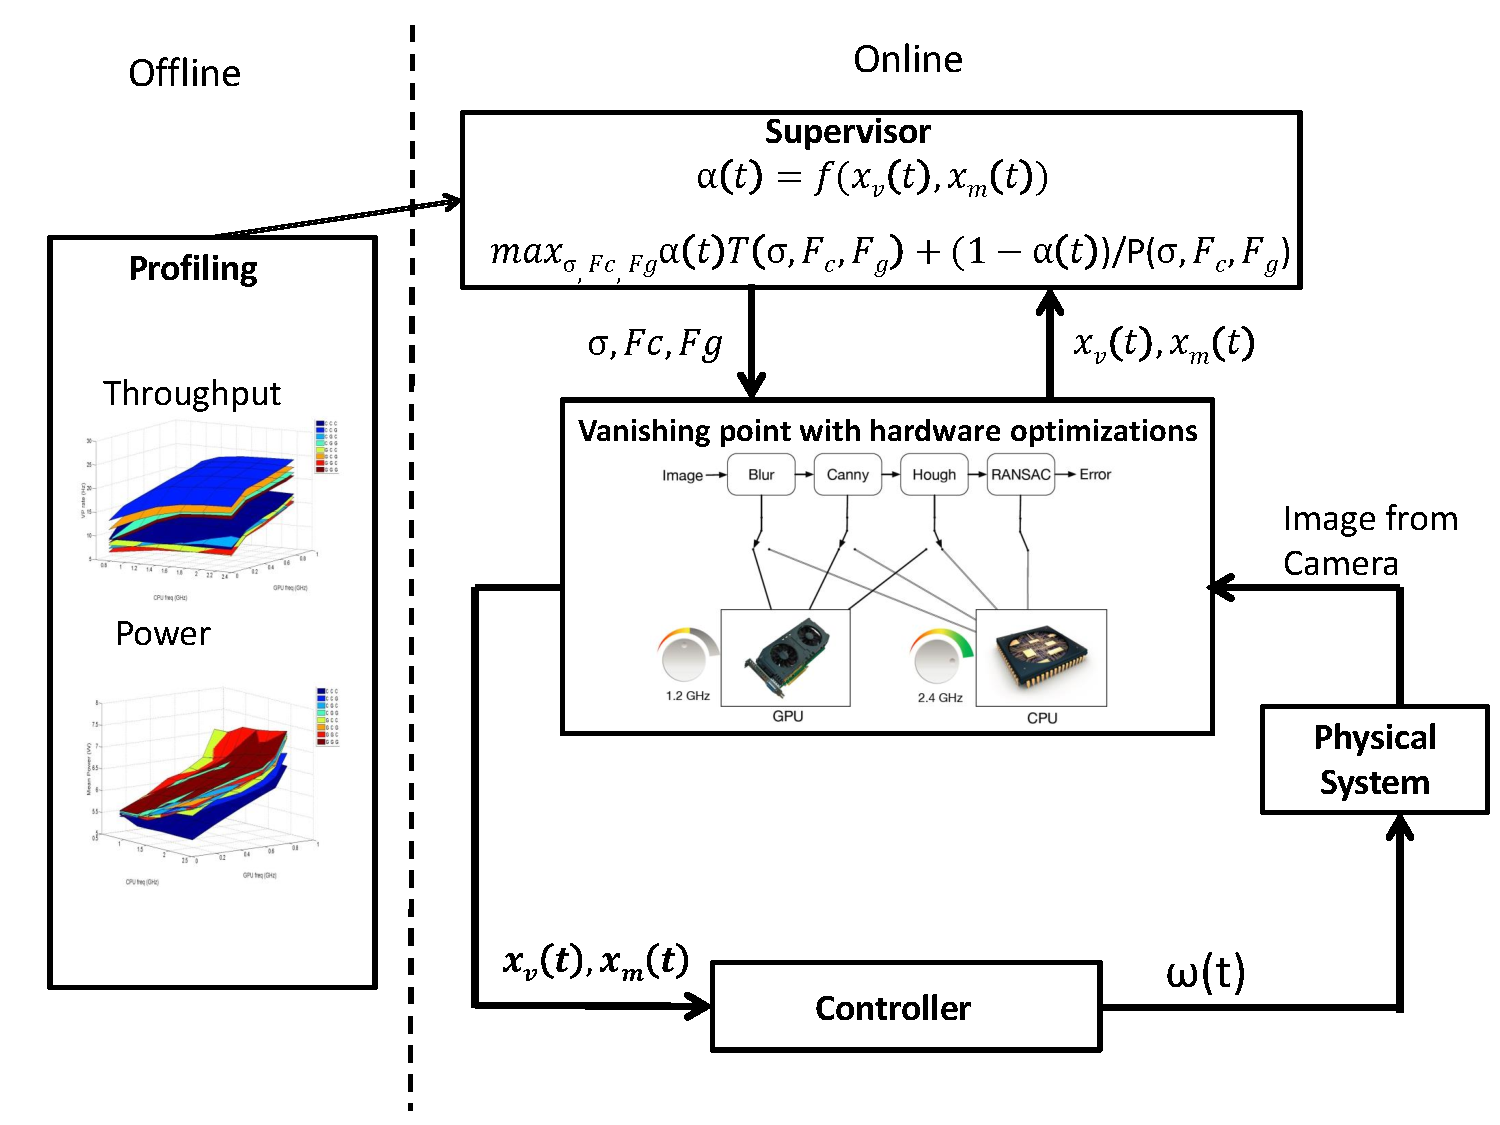
\includegraphics[width=0.46\textwidth]{Figs/bigFig.pdf}
	\vspace{-10pt}
	\caption{Two stage approach.}
	\label{fig:juicyj}%same freq diff assignment}
\end{figure} 

